\section{Signal Modelling}
\label{sec:signalmodelling}

Referred to AN \cite{CMS-PAS-HIG-19-001}

%\subsection{Signal modeling of the SM Higgs}
%\subsubsection{Signal Corrections}
%\label{sec:signalcorr}
%
%For the dominant gluon fusion production mode for the signal, the $p_{\rm T}$ spectrum has been tuned using 
%the ``hfact'' parameter of {\sc powheg} to match closely the Higgs boson $p_{\rm T}$ spectrum in the full phase 
%space as predicted by the {\sc HRes} generator at $\sqrt{s}=13~\TeV$~\cite{powhfact}. The agreement can be seen in Fig.~\ref{fig:PowhegHResPt}. 
%For other mass points, the ``hfact'' parameter is parametrized as a function of $m(\rm{H})$ as hfact$=0.1\cdot m({\rm H})+37.5$.
%
%We use weights defined in bins of generated Higgs pT and number of generated jets to reweight our POWHEG signal sample to the NNLOPS one.
%
%\begin{figure}[!h]
%\centering
%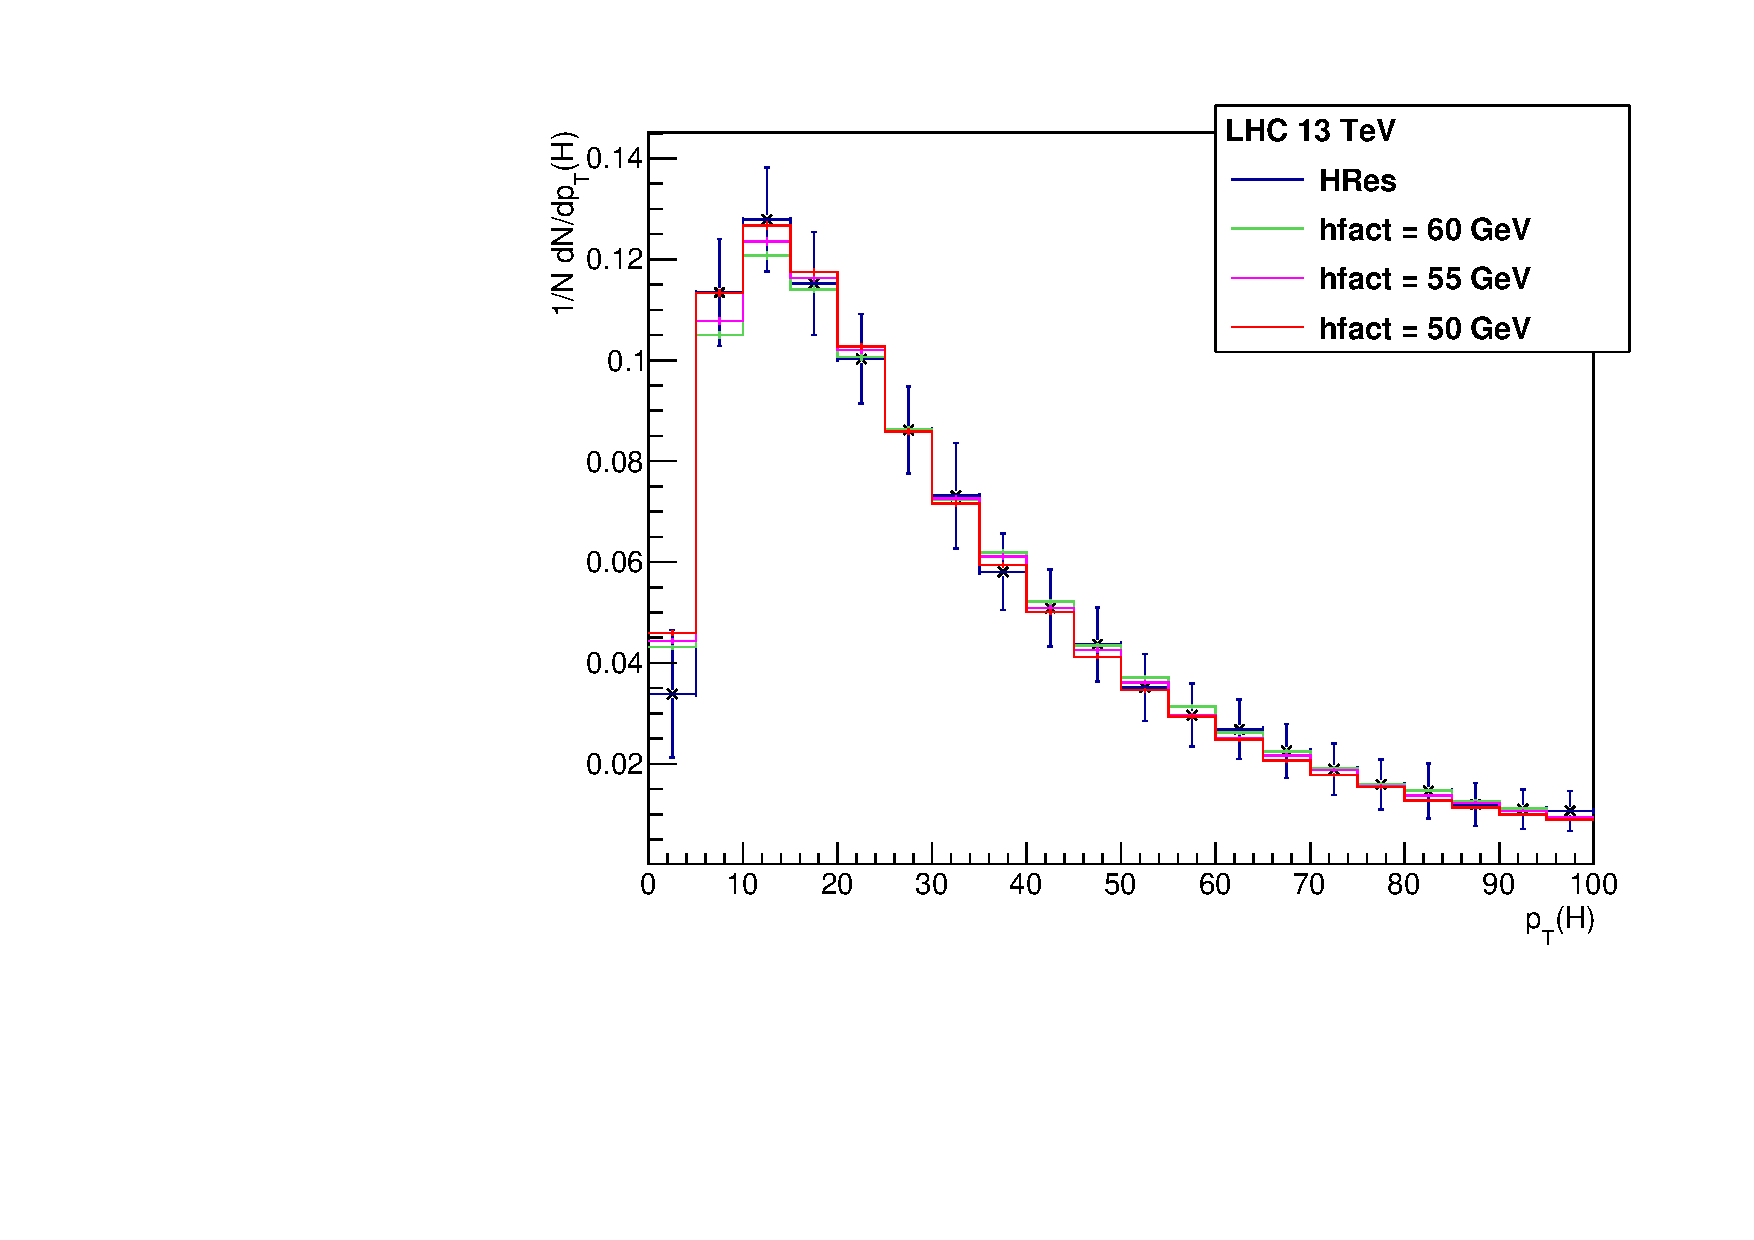
\includegraphics[width=0.6\linewidth]{Figures/Modelling/HResPOWHEGTuning.pdf}
%\caption{Comparison of {\sc powheg} and {\sc HRes} $p_{\mathrm{T}}$ spectrum at 13~\TeV for different hfact. \label{fig:PowhegHResPt}}
%\end{figure}
%
%
%\subsubsection{Signal Normalization}
%\label{sec:signalnorm}
%
%The normalization of the Higgs boson signal in the peak region is directly taken from simulation. Using simulated samples for five $m_H$ points (120, 124, 125, 126 and 130 GeV), polynomial fits of the expected signal yields in a $[105, 140]$ GeV $\mllll$ window around the Higgs boson peak are performed.
%%separately for the stage 1.2 bins, in the three final states and the twenty two categories. 
%%Some examples of the fits are shown in Fig.~\ref{fig:signalyieldfits} for the different stage 1.2 bins. 
%
%%\begin{figure}[!h]
%%\centering
%%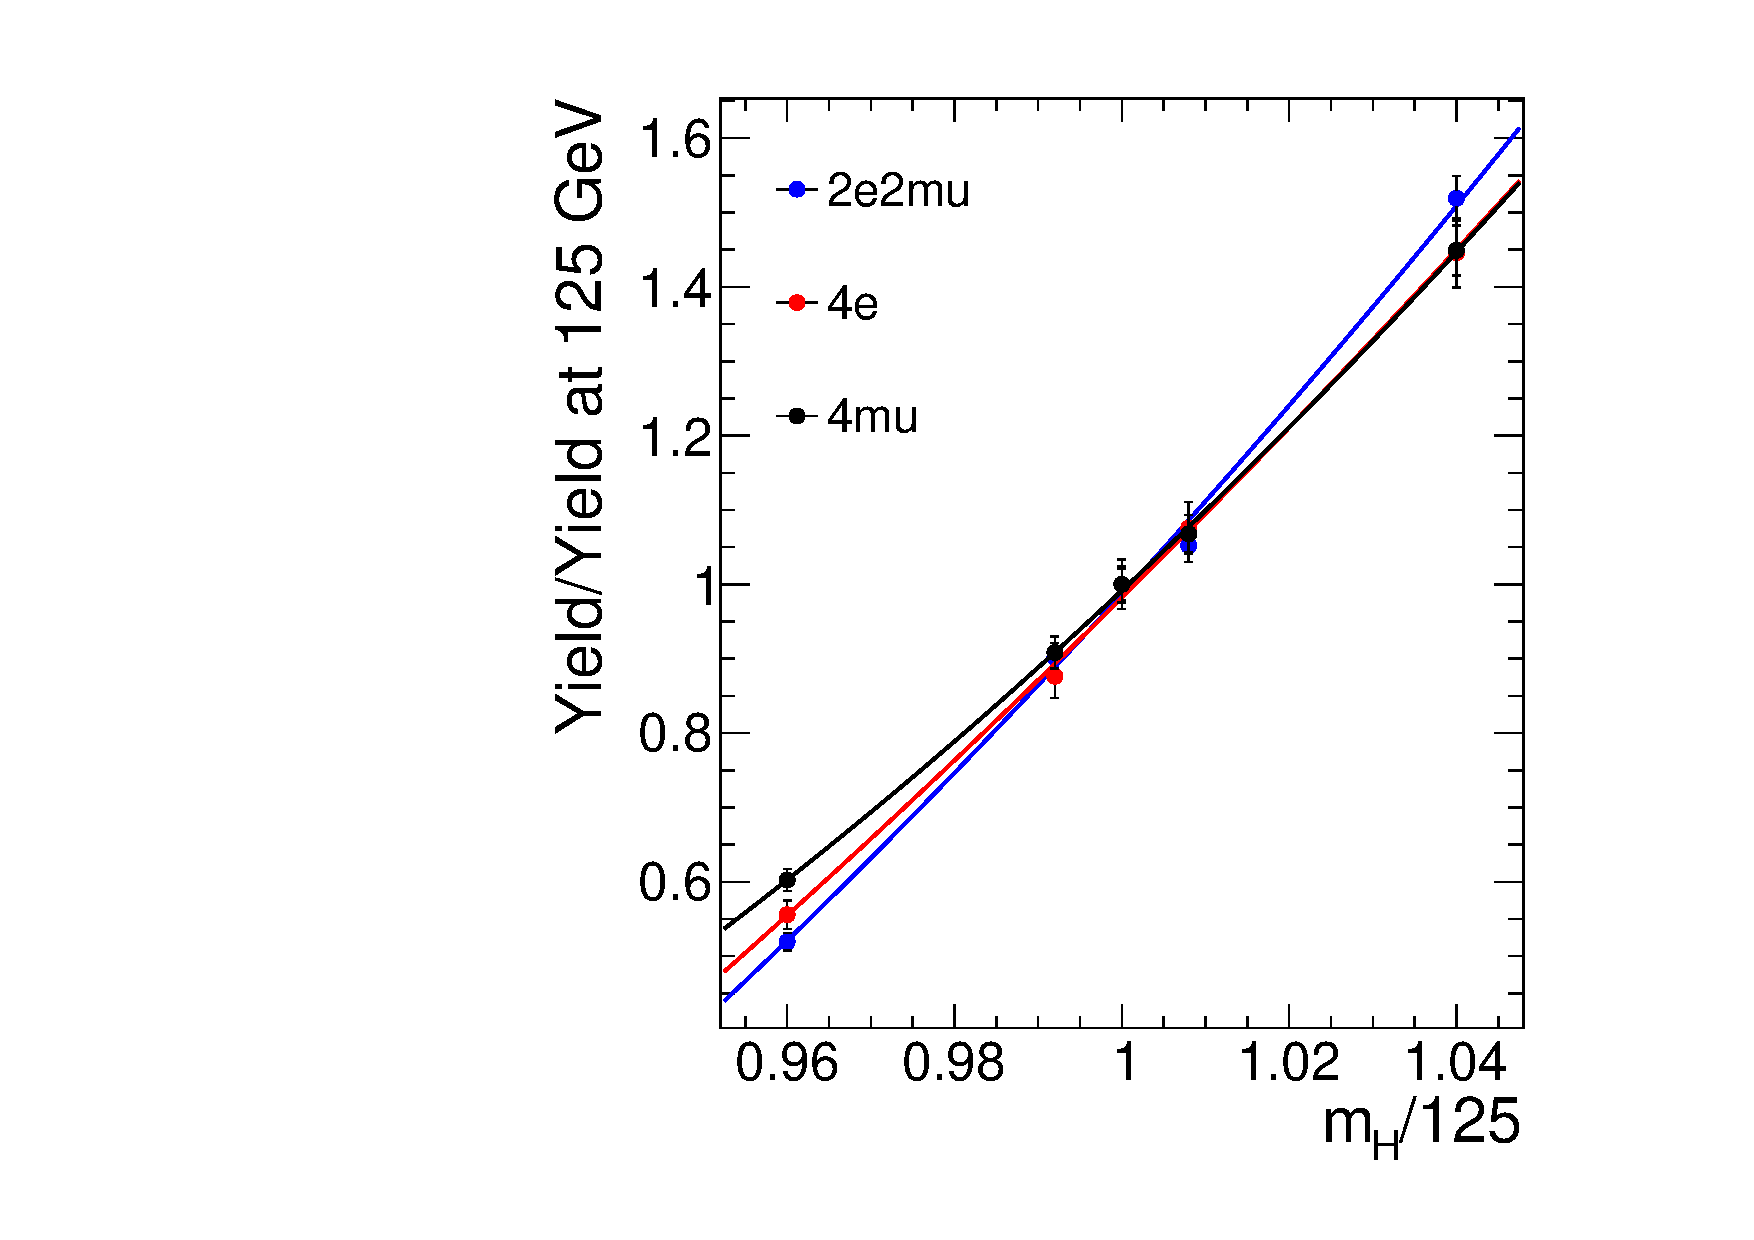
\includegraphics[width=0.25\linewidth]{Figures/Signal/fit_ggH_1j_60_120_ggH_1j_60_120_2018.pdf}
%%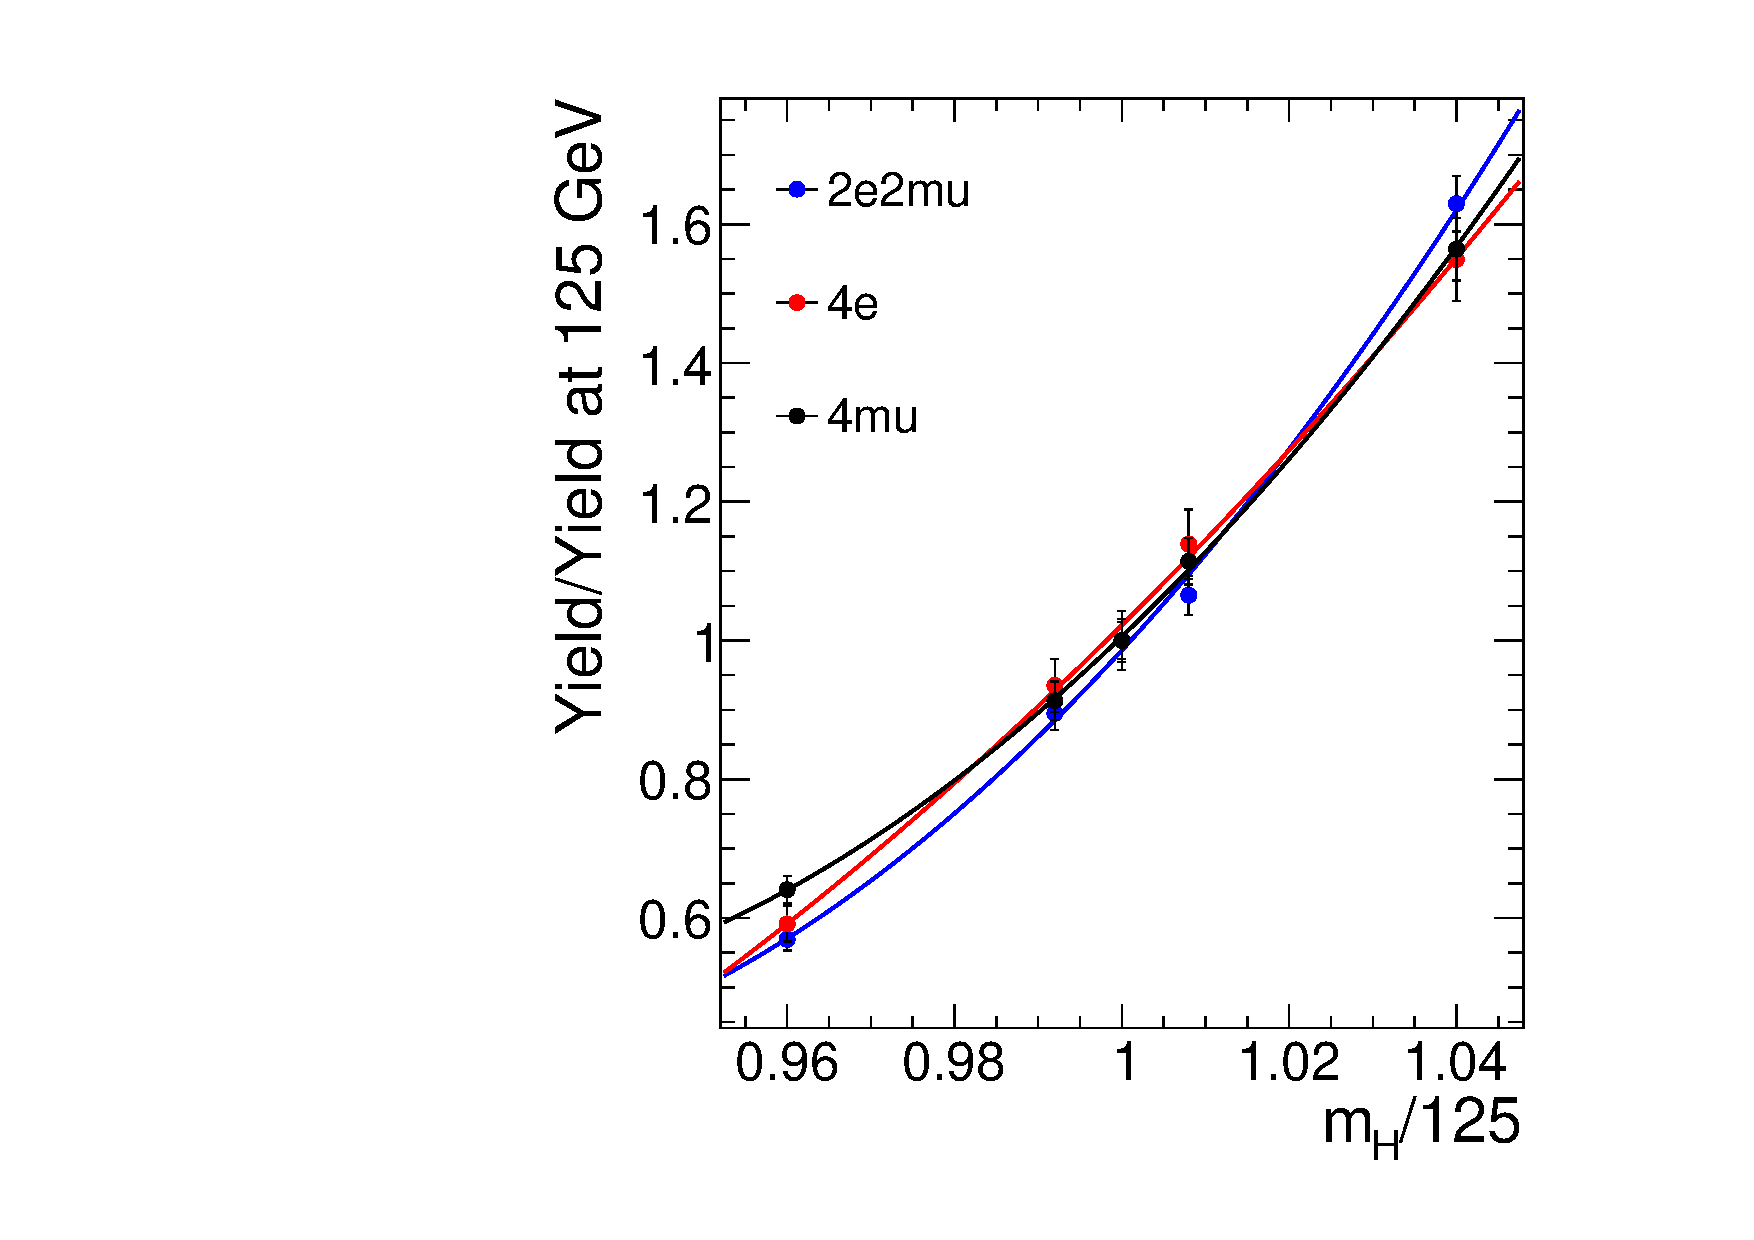
\includegraphics[width=0.25\linewidth]{Figures/Signal/fit_VBF_1j_ggH_1j_60_120_2018.pdf}\\
%%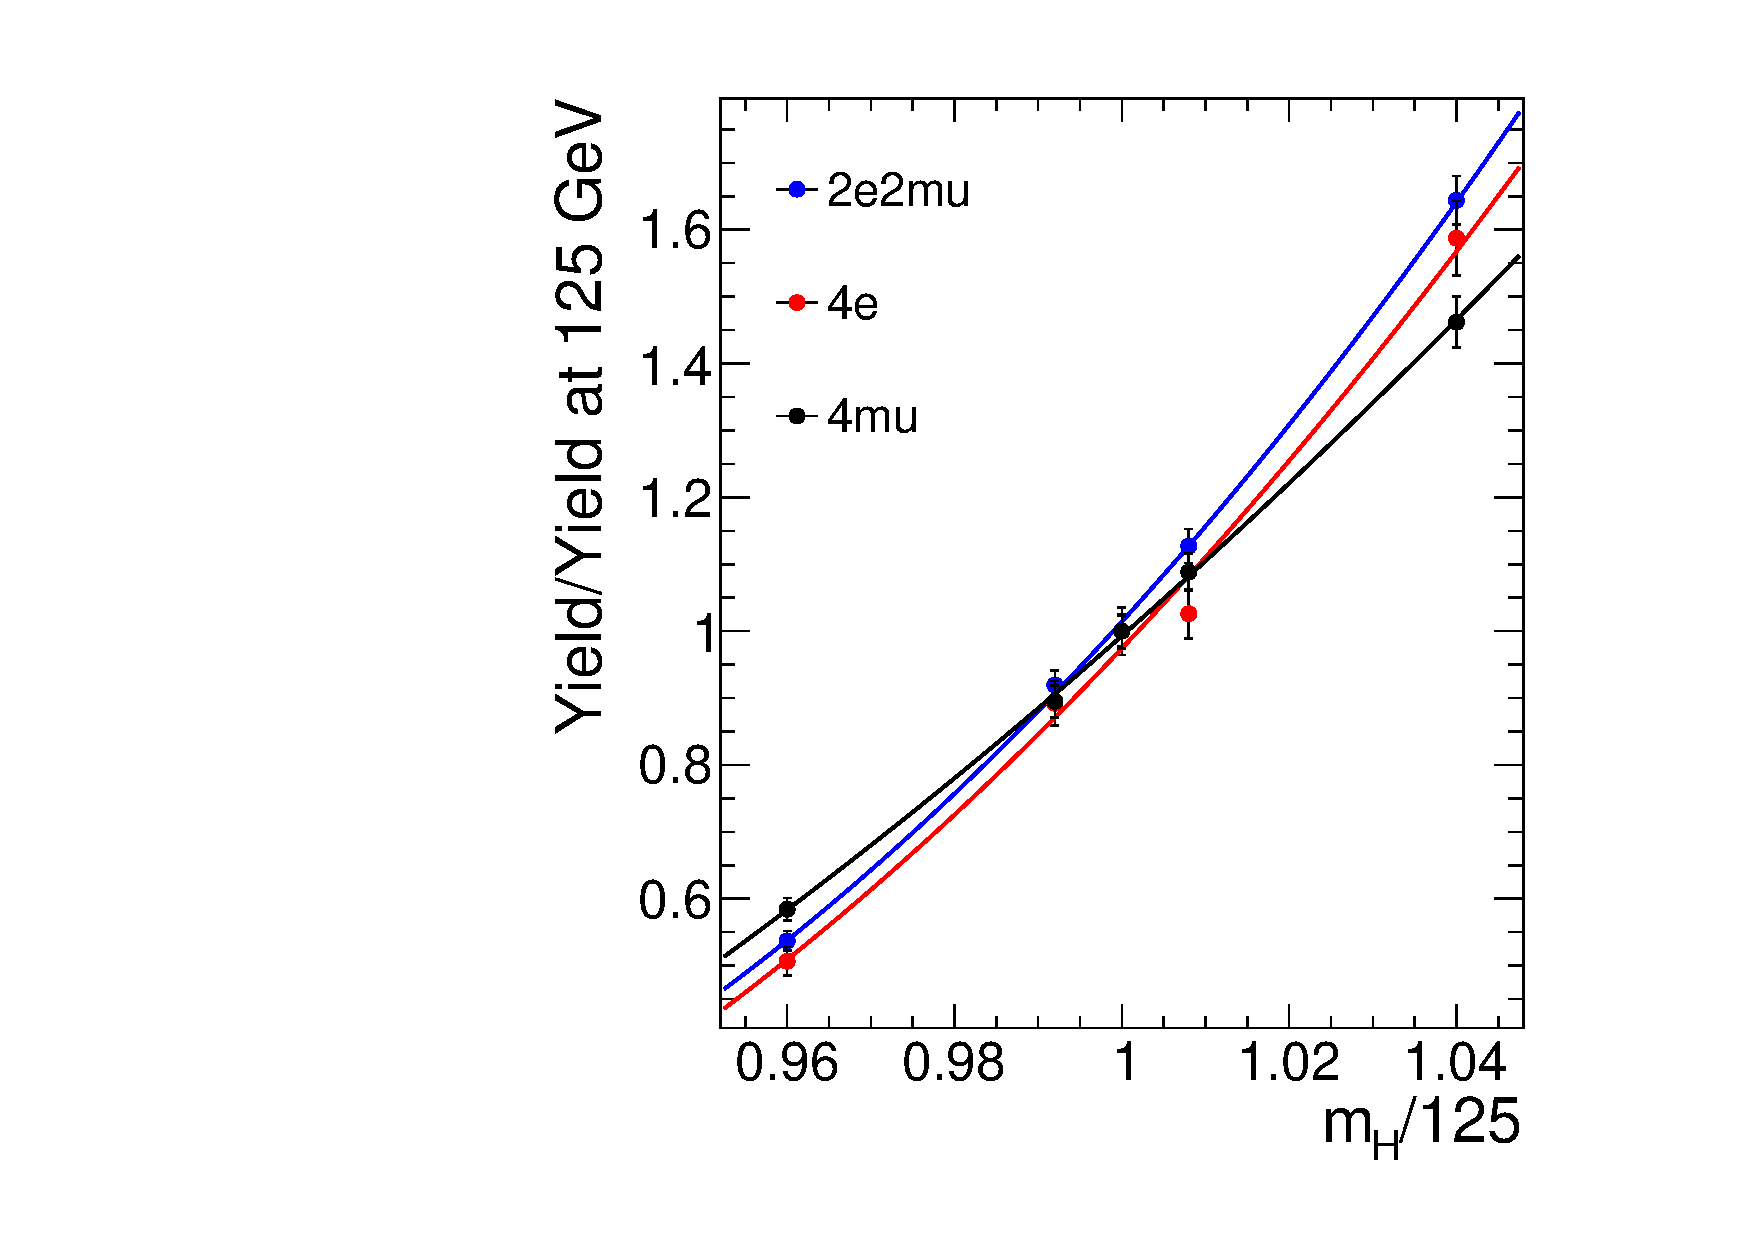
\includegraphics[width=0.25\linewidth]{Figures/Signal/fit_ggH_1j_0_60_VBF_Rest_2018.pdf}
%%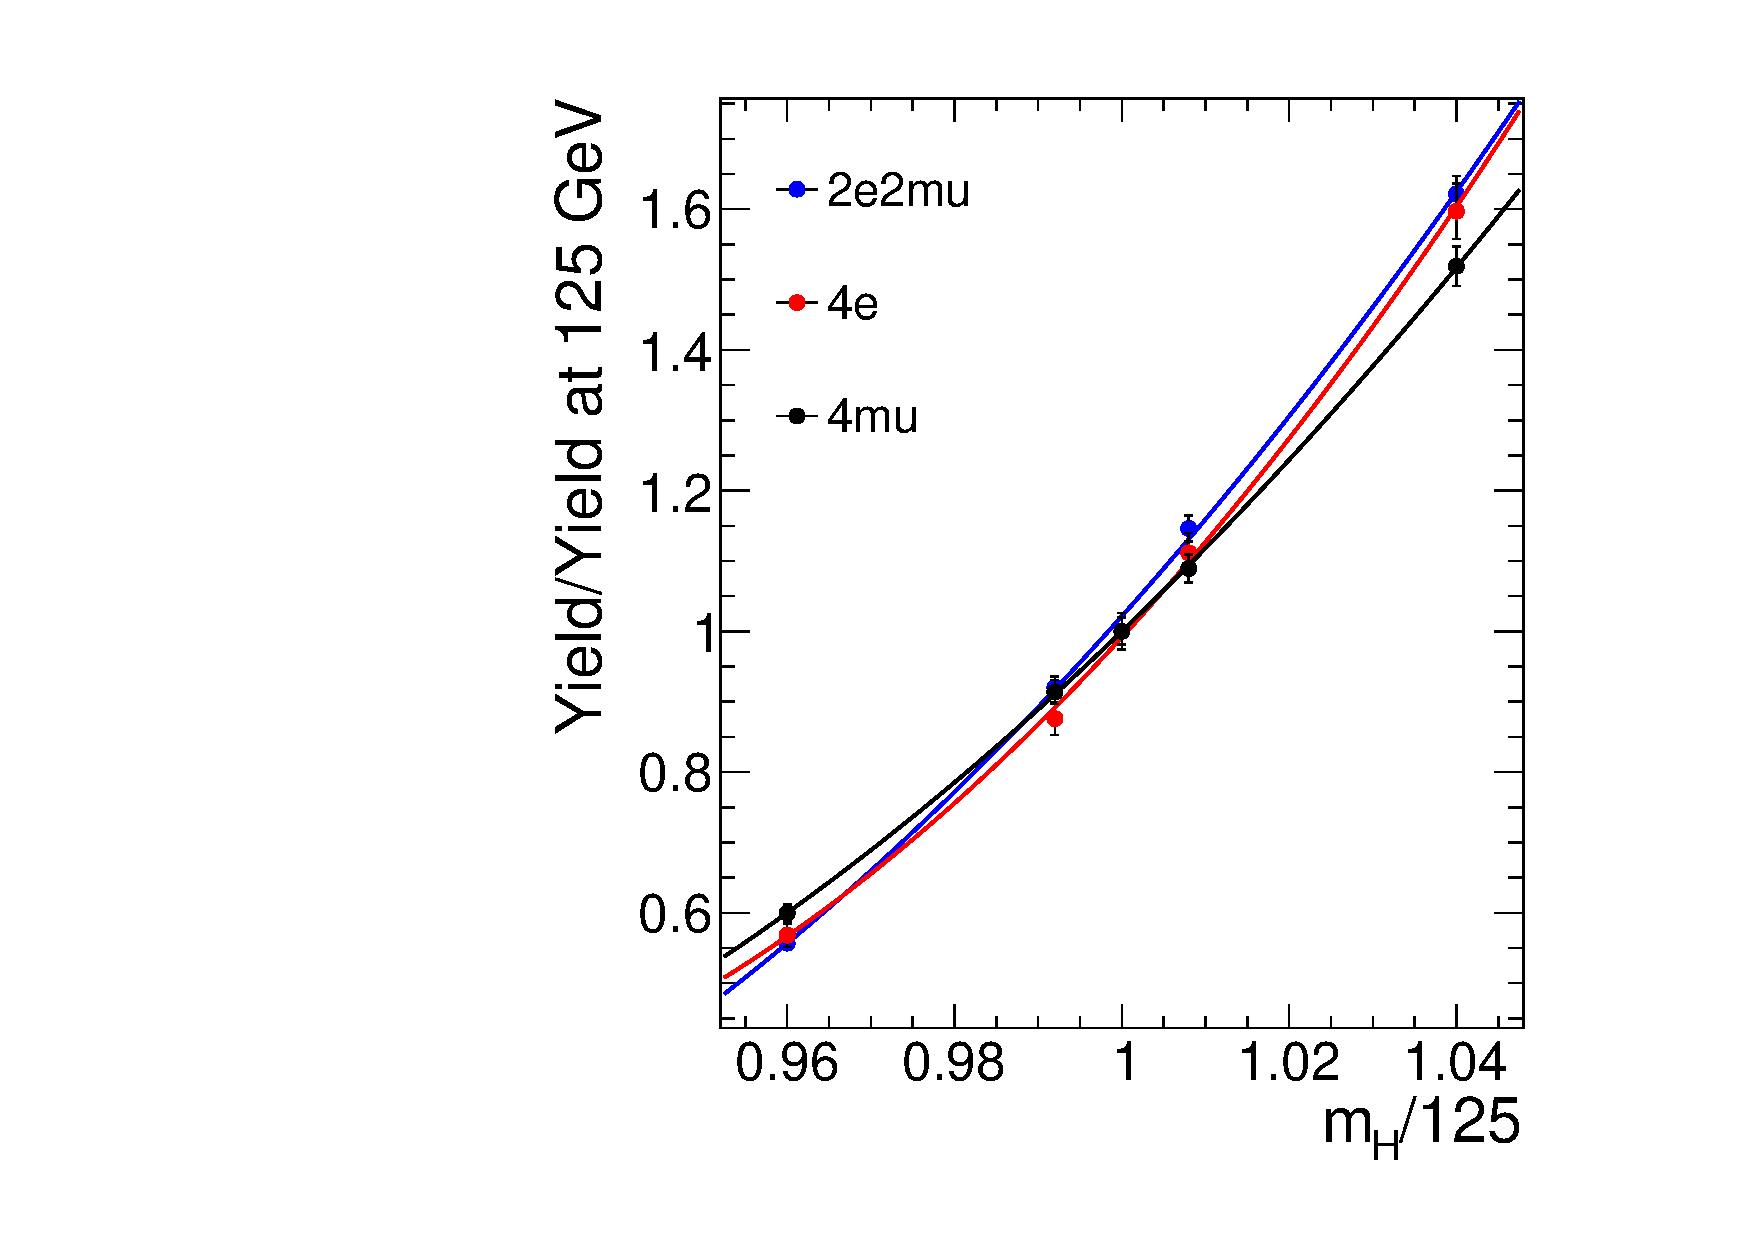
\includegraphics[width=0.25\linewidth]{Figures/Signal/fit_VBF_1j_VBF_Rest_2018.pdf}\\
%%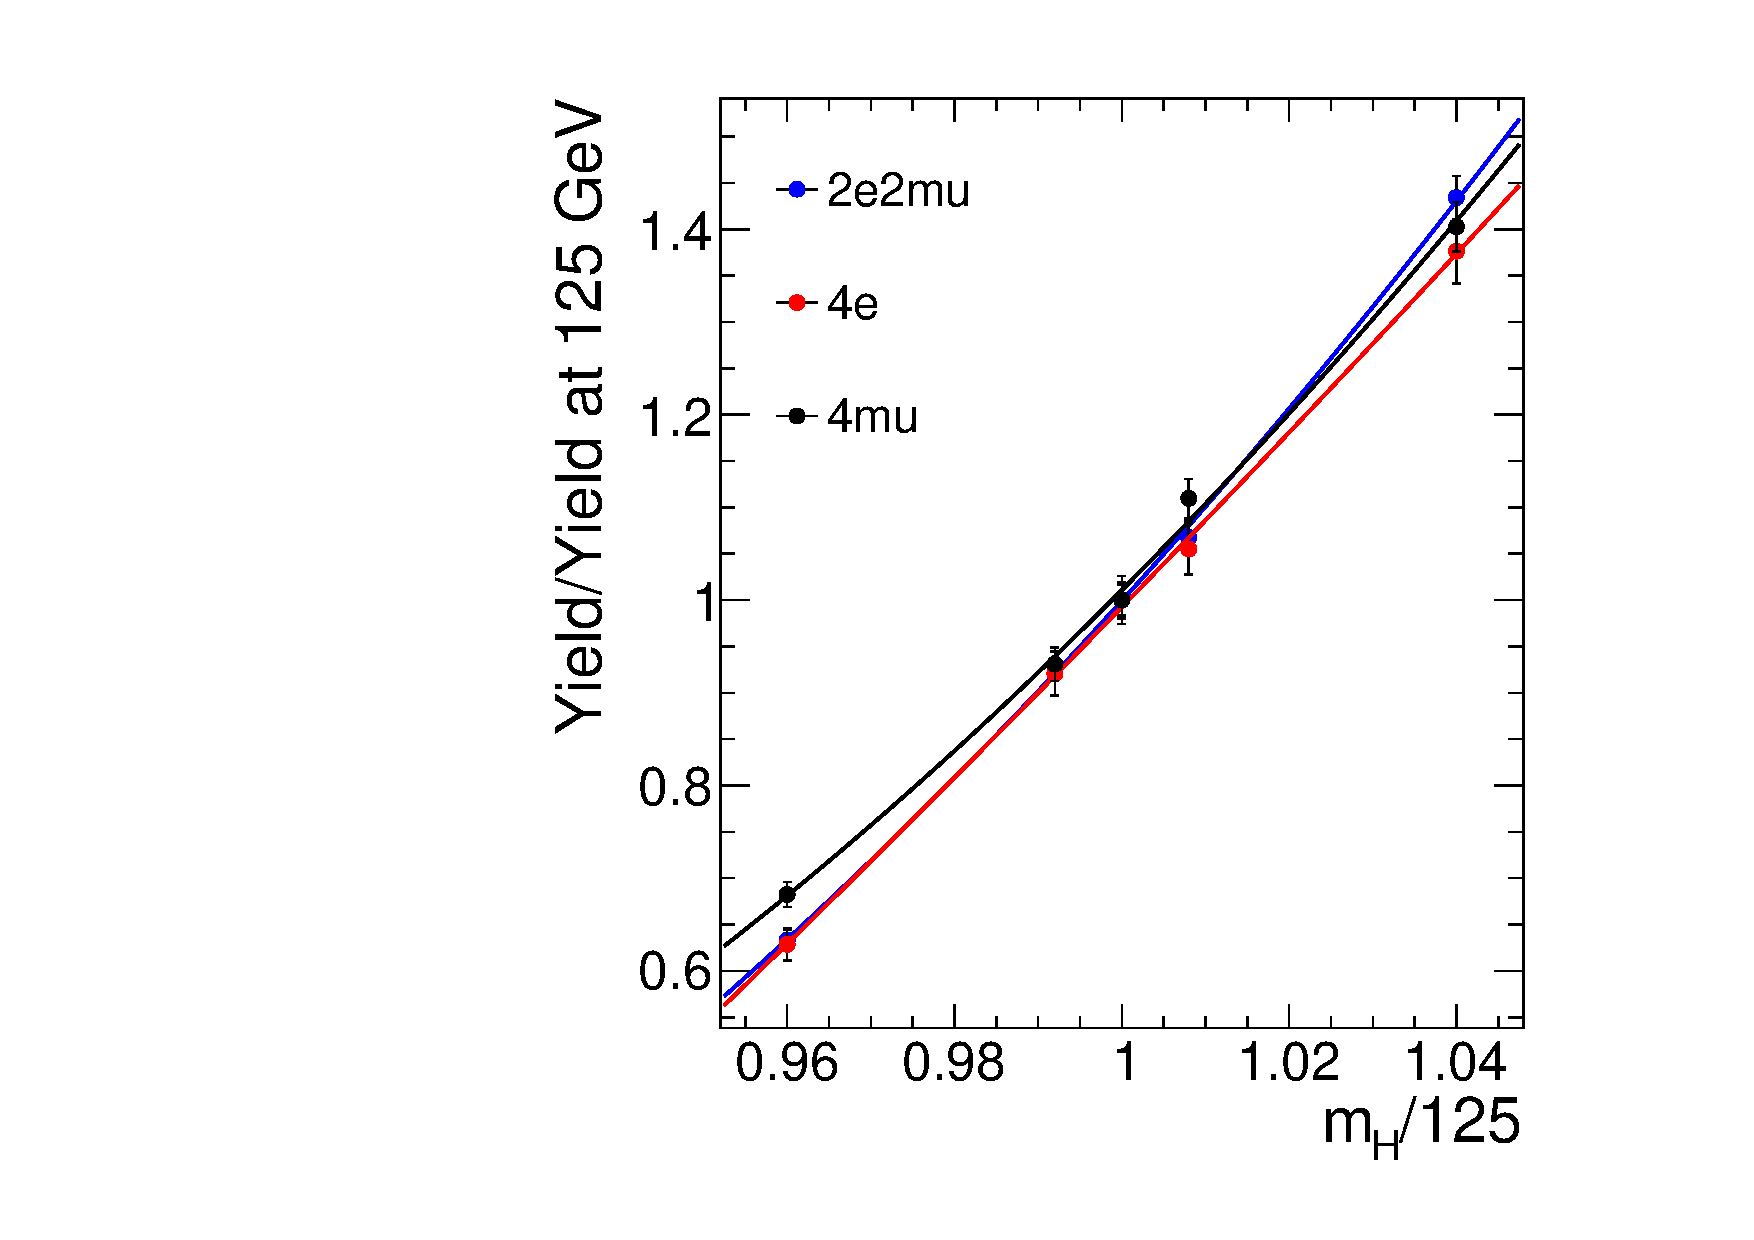
\includegraphics[width=0.25\linewidth]{Figures/Signal/fit_VH_Lep_0_150_VH_Lep_0_150_2018.pdf}
%%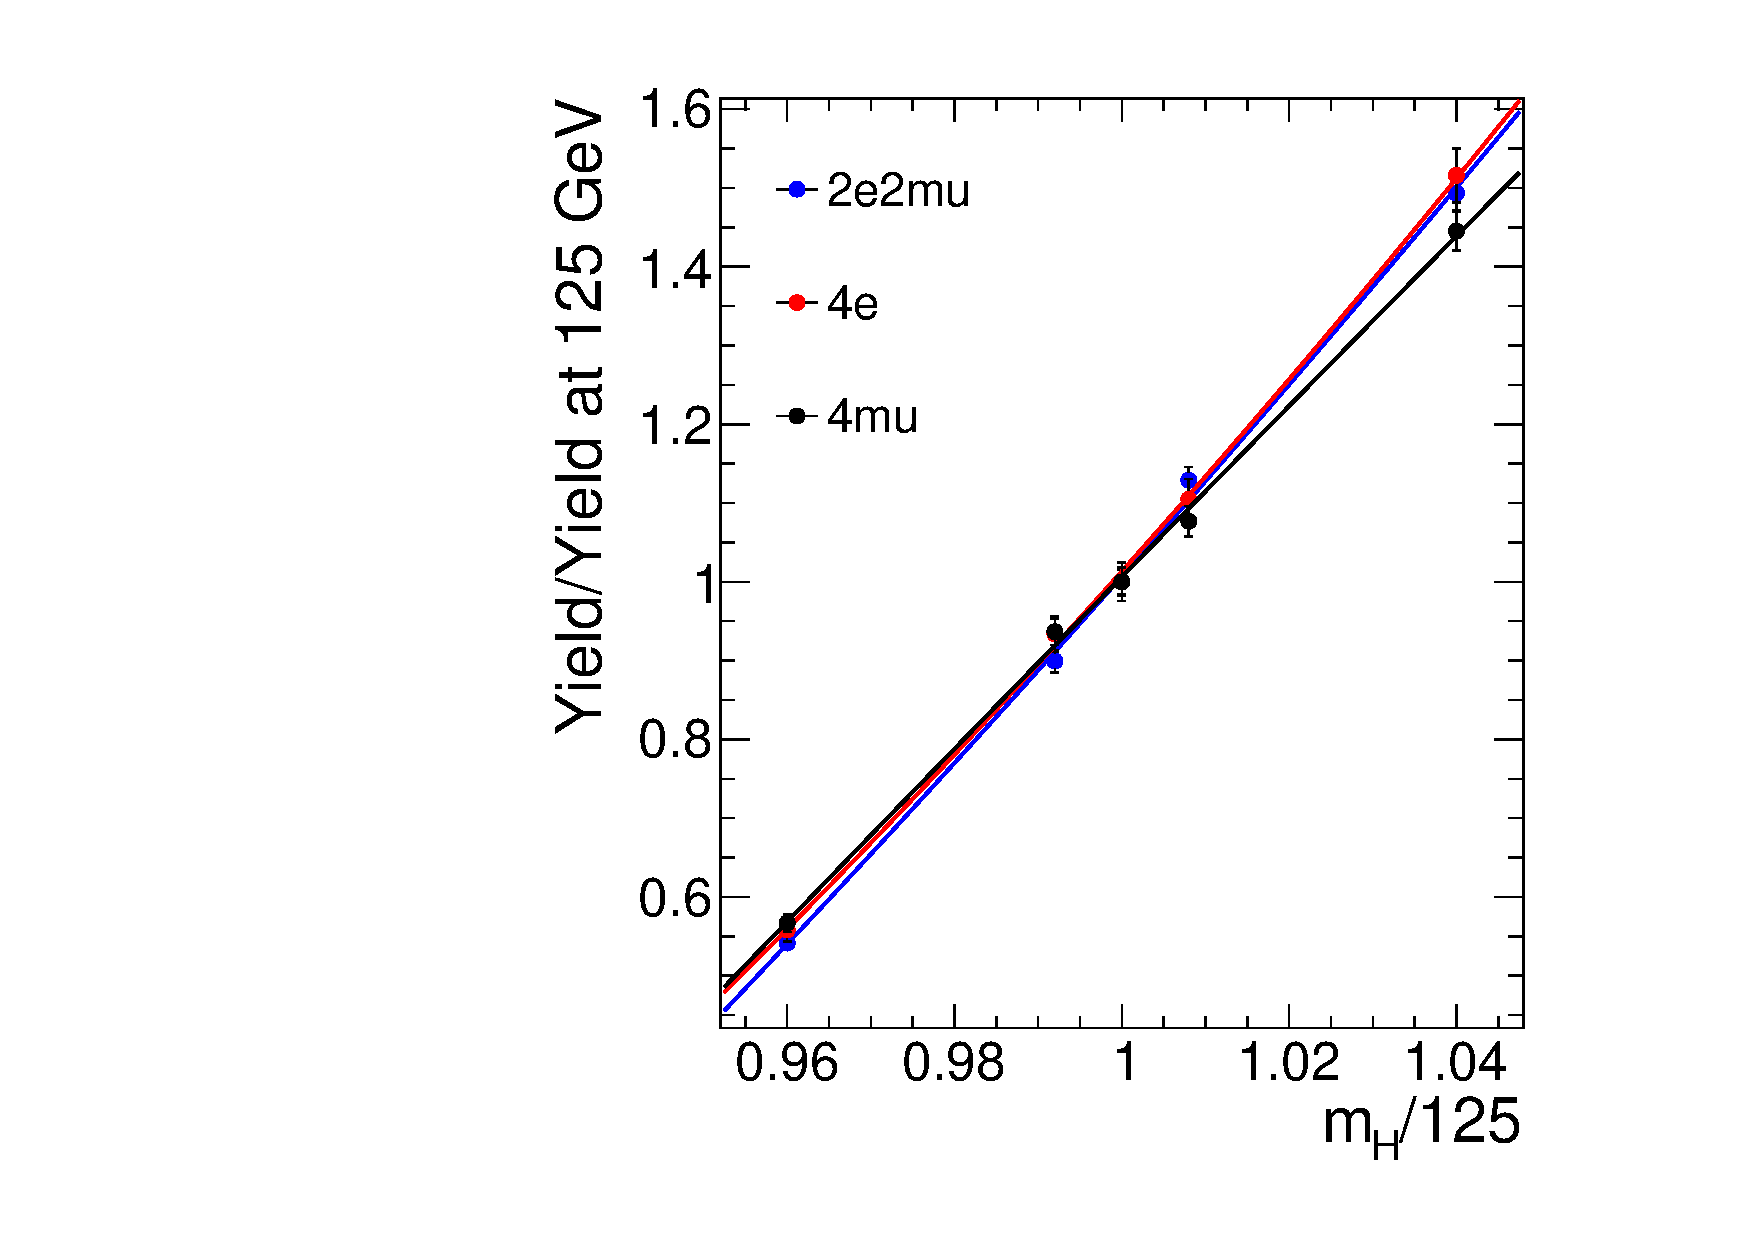
\includegraphics[width=0.25\linewidth]{Figures/Signal/fit_VH_Had_VH_Had_2018.pdf}\\
%%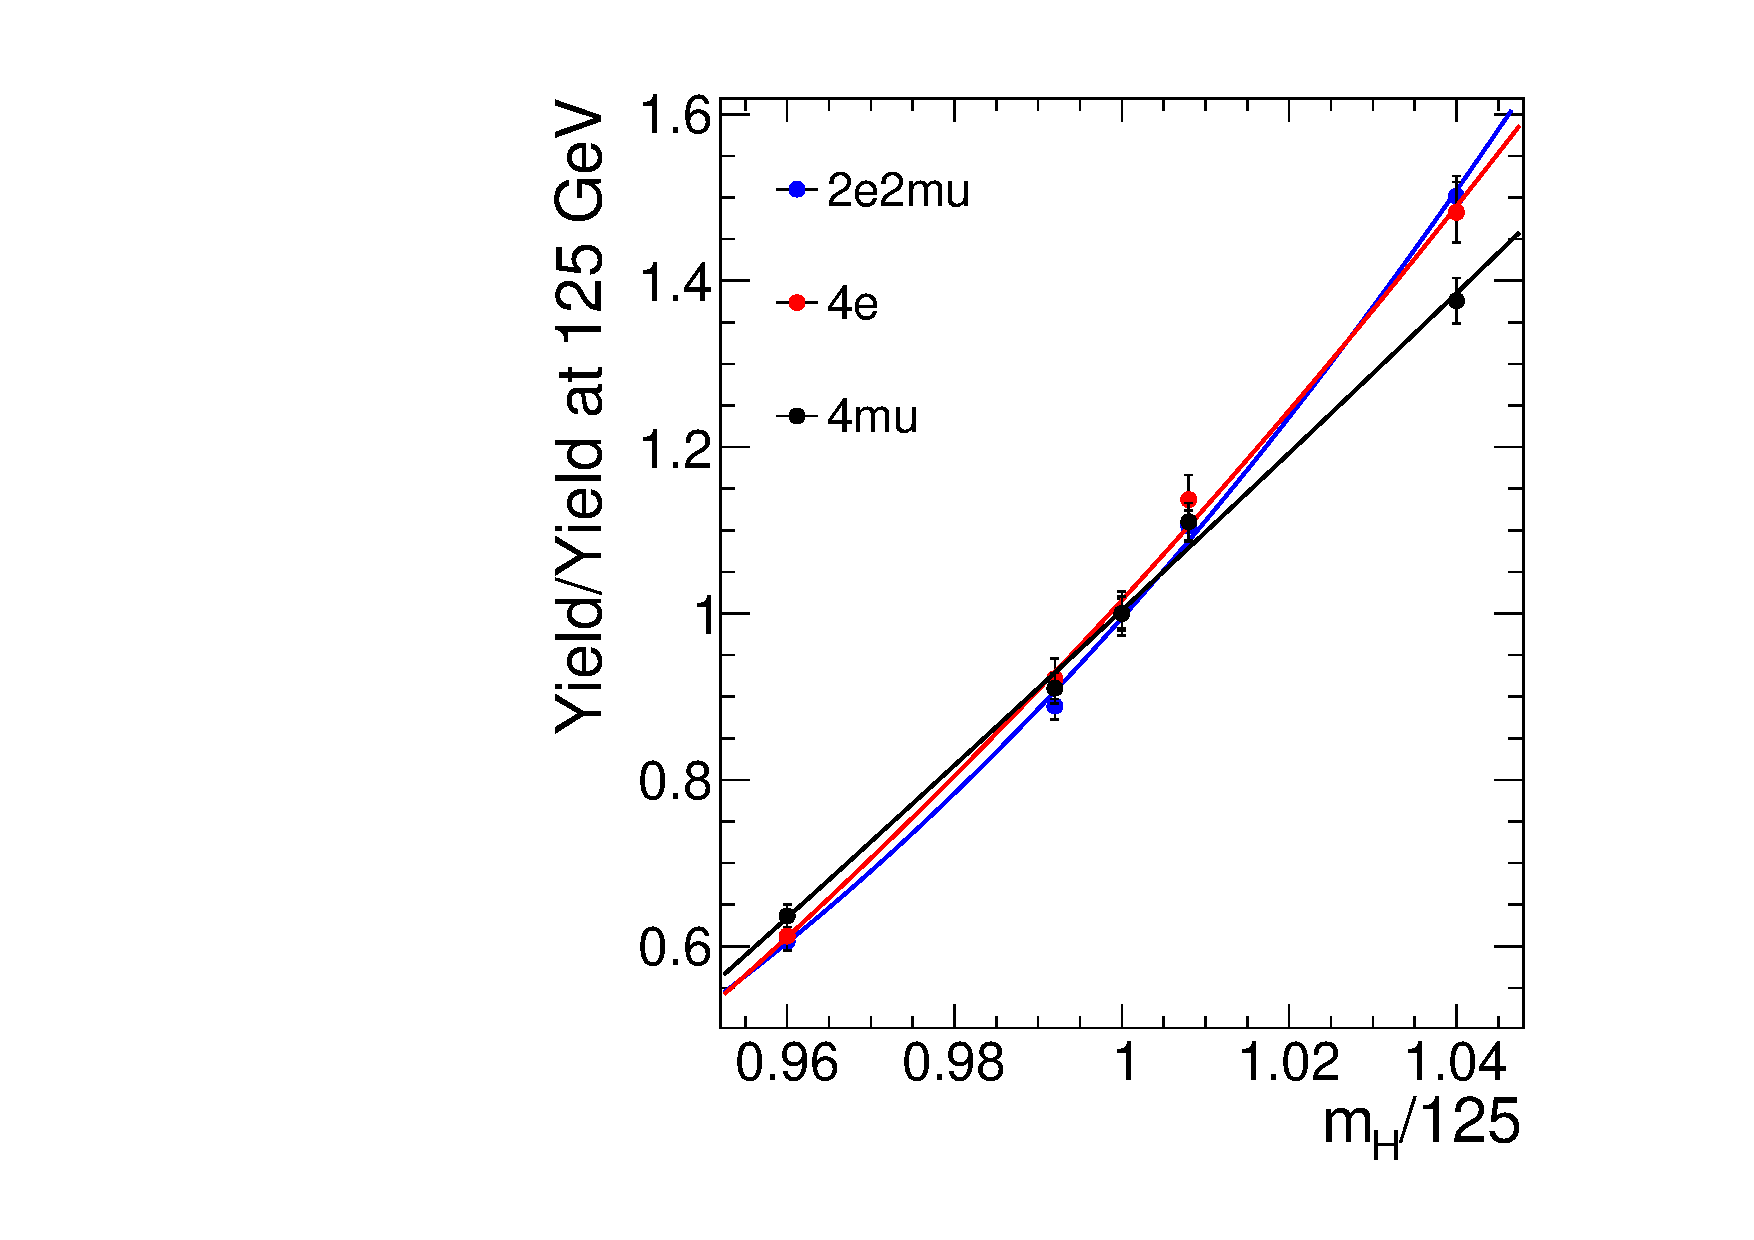
\includegraphics[width=0.25\linewidth]{Figures/Signal/fit_TTH_Had_TTH_2018.pdf}
%%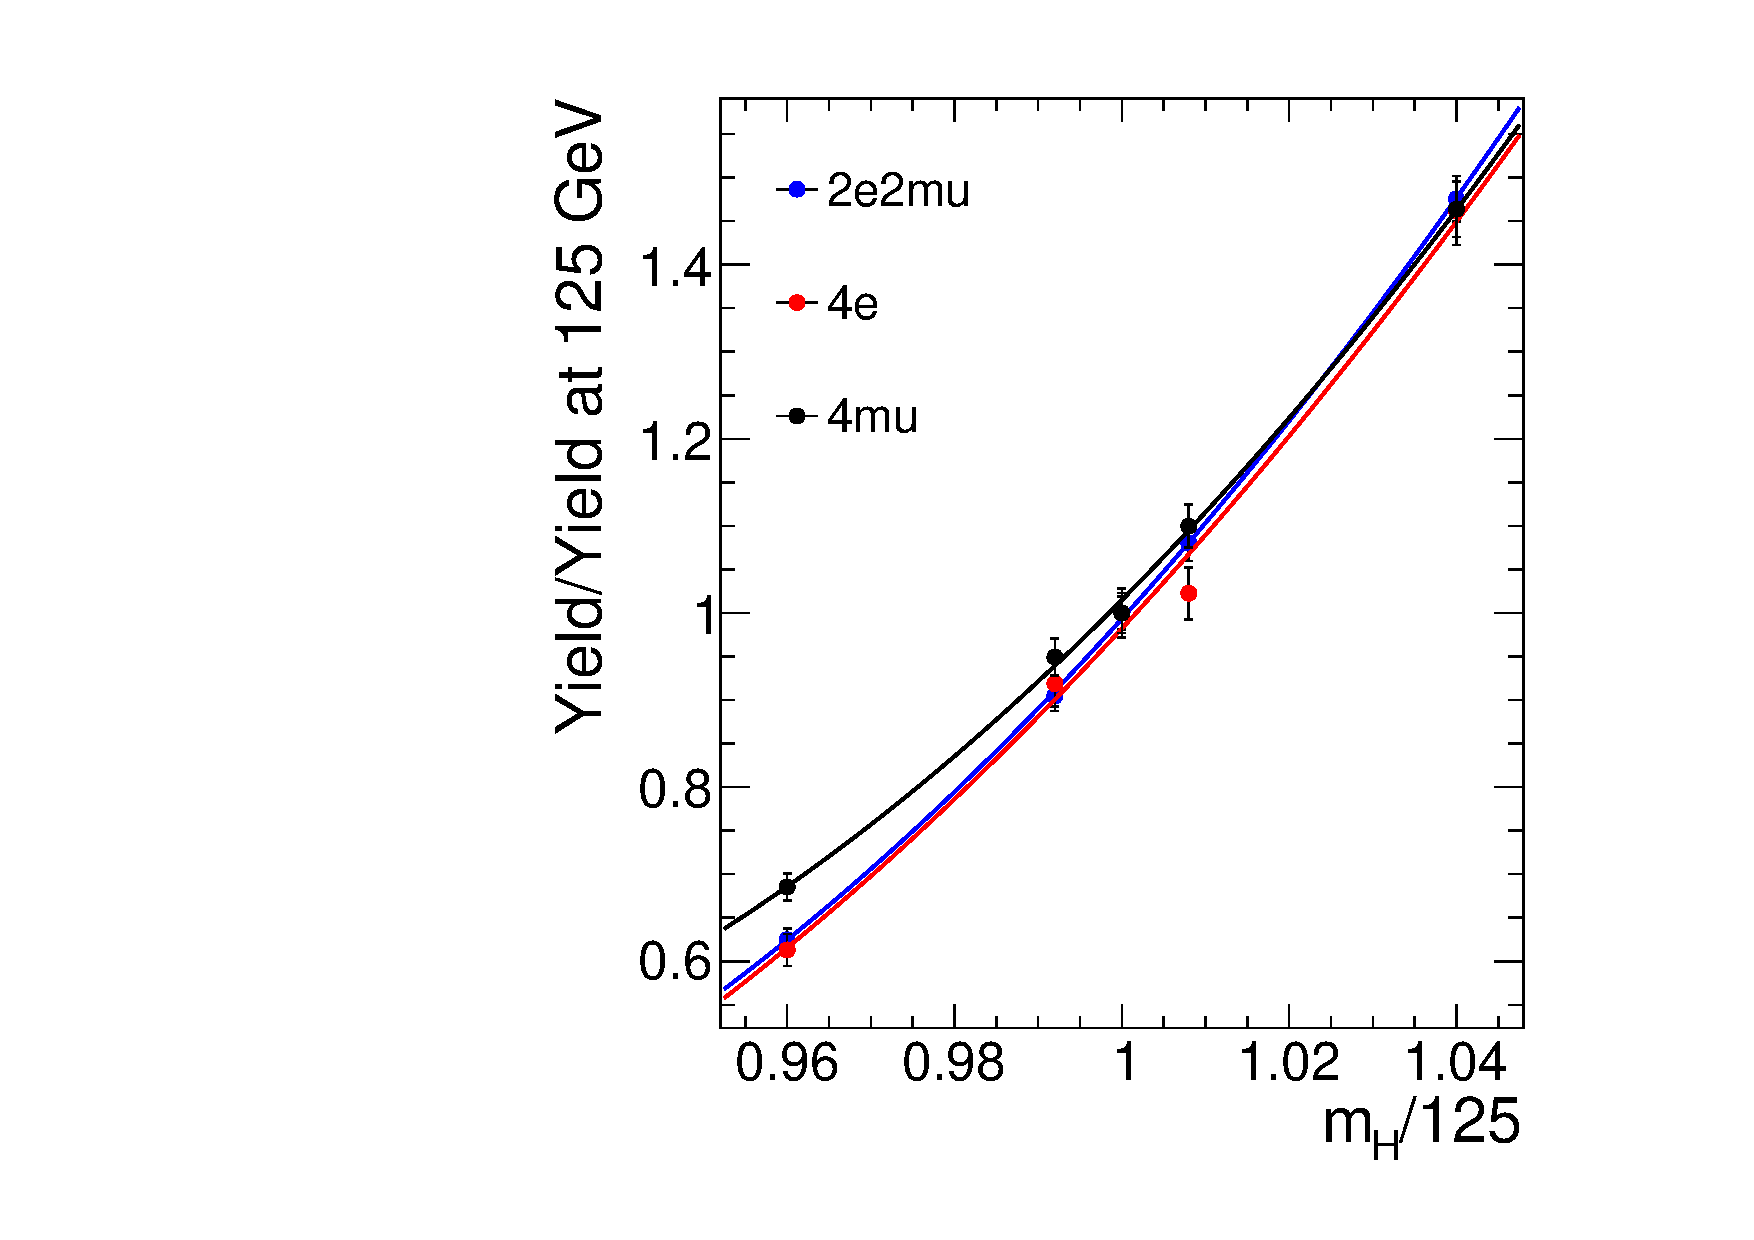
\includegraphics[width=0.25\linewidth]{Figures/Signal/fit_TTH_Lep_TTH_2018.pdf}\\
%%\caption{Fits of the expected signal yields after full event selection in a $[105, 140]$ GeV $\mllll$ window, for the ggH\_1j\_60\_200 stage 1.2 bin in ggH\_1j\_60\_200 and VBF\_1j categories(rows 1), VBF\_Rest stage 1.2 bins in ggH\_1j\_0\_60 and VBF 1jet categories (row 2), VH-hadronic and VH-leptonic (row 3) in their dedicated categories and ttH production mode in ttH hadronic and leptonic categories (row 4) in the $[118, 130]$ GeV range of generated $m_H$. %\textbf{Fits currently done on the few mass points currently available}
%%}
%%\label{fig:signalyieldfits}
%%\end{figure}
%
%\clearpage
%
%\subsubsection{Signal Lineshape}
%\label{sec:signalshapes}
%
%In this section we describe the PDF used to describe the signal shapes 
%for different masses  in different Event Categories as explained before. 
%The resolution function model depends only on the leptons quality, while the exact 
%shape depends on the lepton kinematics, and so depend also on the Higgs mass. A Double
%Crystal-Ball function $f_{dCB}(m_{4\ell} \, | \, m_{H})$:
%%
%\begin{equation}
%dCB(\xi ) = N \cdot \left\{ {\begin{array}{*{20}c}
%   { A \cdot \left( B  + |\xi | \right)^{- n_L } ,  {\rm{      \,\,\,\,   for \,\, }} \xi  < \alpha_L }  \\
%   { A \cdot \left( B  + |\xi | \right)^{- n_R } ,  {\rm{      \,\,\,\,   for \,\, }} \xi  > \alpha_R }  \\
%   {\exp \left( - \xi ^2  / 2 \right) ,            {\rm{      \,\,\,\,   for  \,\, }} \alpha_L \leq \xi  \leq \alpha_R }  \\
%\end{array}} \right.
%\label{eq:dCB}
%\end{equation}
%%
% 
%where $ \xi = ( m_{4\ell} - m_{H} - \Delta m_{H} ) /\sigma_m$.
%This function has six independent parameters, and is intended to
%capture the Gaussian core ($\sigma_m$) of the four-lepton mass
%resolution function, systematic mass shift $\Delta m_{H}$ of the
%peak, and the left- and right-hand tail originating from leptons
%emitting brem in the tracker material, present for both electrons and
%muons, and from the non-Gaussian mis-measurements specific to
%interactions of electrons with the detector material (two parameters,
%$n$ and $\alpha$, for each side of the mean): The prominence of the
%left-,right-hand tail is defined the power $n_L$, $n_R$, respectively.
%The parameters $\alpha_L$, $\alpha_R$ define where the splicing of the
%tails and the core are made, in units of $\sigma_m$. Parameters $A$ and $B$ are not
%independent; they are defined by requiring the continuity of the
%function itself and its first derivatives.  $N$ is the normalizing
%constant.
%
%%We model each stage 1.2 bin shapes in three final states at various mass points (120-130). 
%The fitting strategy used to deal with this situation is to use the linear approximation
%of all the Double Crystal Ball parameters varying with  with $m_{H}$.
%
%%
%\begin{equation}
%	params = parms_{CB0} + params_{CB1} \times (m_{H} -125 GeV) + params_{CB2} \times (m_{H} -125 GeV) ^2 
%\label{eq:linear}
%\end{equation}
%%
%Simultaneous fits are performed using 5 mass samples to extract the $parms_{CB0}$, $params_{CB1}$ and $params_{CB2}$. The initial value for the $parms_{CB0}$ is obtained by fitting 125 GeV mass sample alone, and refitted in the simultaneous fits.
%%Some examples of the fits are shown in Fig.~\ref{fig:sigShapeFits13TeV125} and~\ref{fig:sigShapeFits13TeV12xx5} for the ggH and $VH$ Stage 1.2 bins. The simultaneous fit at different mass points are shown in Fig.~\ref{fig:simFitVBF}. 
%\begin{figure}[!h]
%\centering
%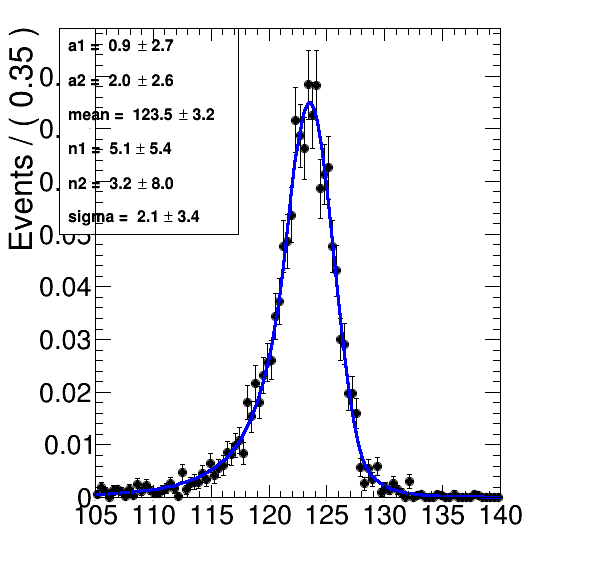
\includegraphics[width=0.32\linewidth]{Figures/Signal/fit_stage_ggH_0j_0_10_4e2018.png} % ZHfitM125__4e_UntaggedMor18} 
%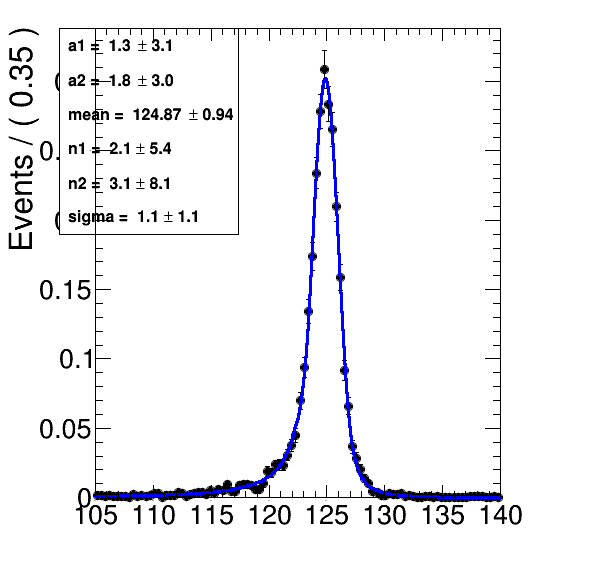
\includegraphics[width=0.32\linewidth]{Figures/Signal/fit_stage_ggH_0j_0_10_4mu2018.png} %ZHfitM125__4mu_UntaggedMor18} 
%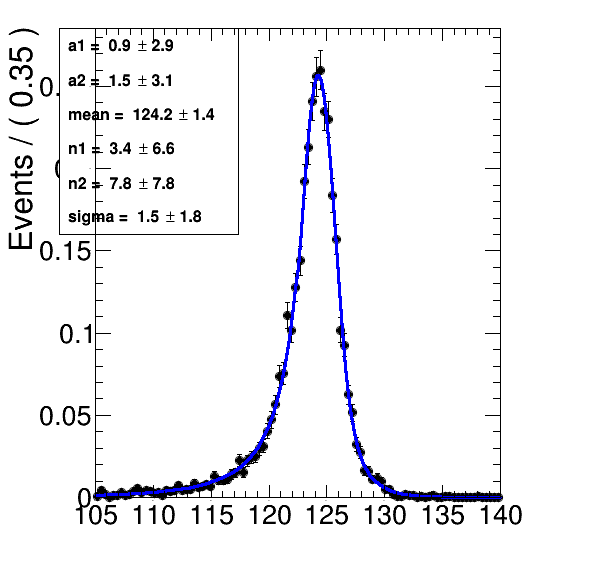
\includegraphics[width=0.32\linewidth]{Figures/Signal/fit_stage_ggH_0j_0_10_2e2mu2018.png} %ZHfitM125__2e2mu_UntaggedMor18} \\ %fitM125_ggH_4e_UntaggedMor18.png} %fitM125_ggH_2e2mu_UntaggedMor18.png} \\
%\caption{Probability density functions $f(m_{4l}|m_{H})$ for signal
%  with {\bf $m_H$=125 \GeV} at the reconstruction level after the full lepton and event selections are applied. The distributions obtained {\bf from 13\TeV} ggH  MC samples are fitted with the model described in the text for  $4\mu$ (left), $4e$ (center) and $2e2\mu$ (right) events. The distribution show the events in the stage 1.1 bin ggH\_0j\_0\_10.  
%\label{fig:sigShapeFits13TeV125}}
%\end{figure}
%
%%\begin{figure}[!h]
%%\centering
%%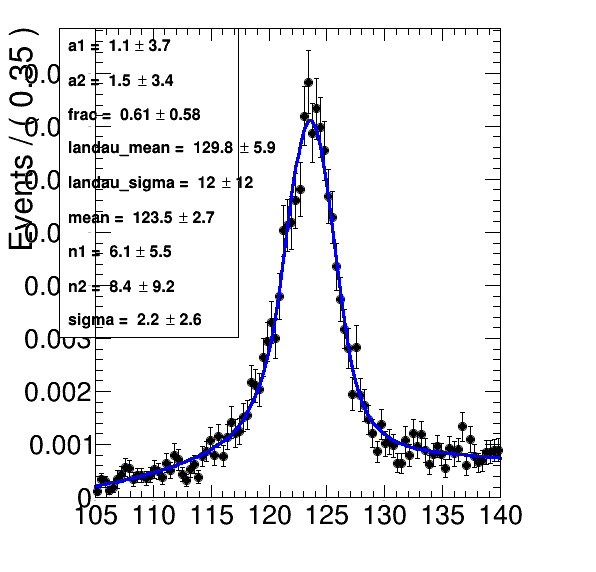
\includegraphics[width=0.32\linewidth]{Figures/Signal/fit_stage_VH_Lep_0_150_4e2018.png} 
%%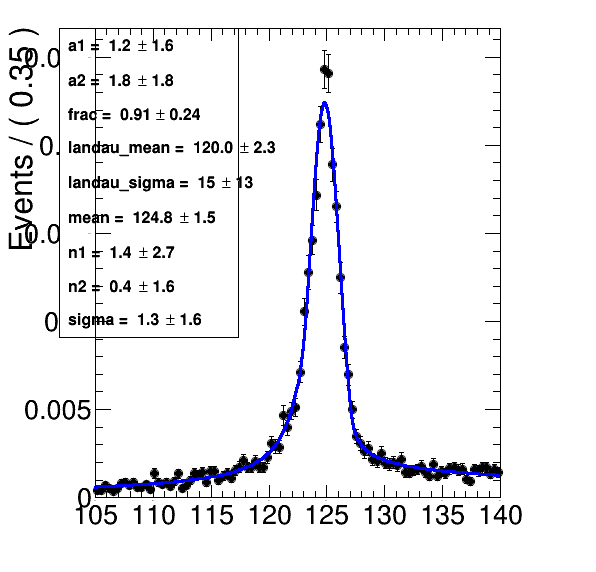
\includegraphics[width=0.32\linewidth]{Figures/Signal/fit_stage_VH_Lep_0_150_4mu2018.png} 
%%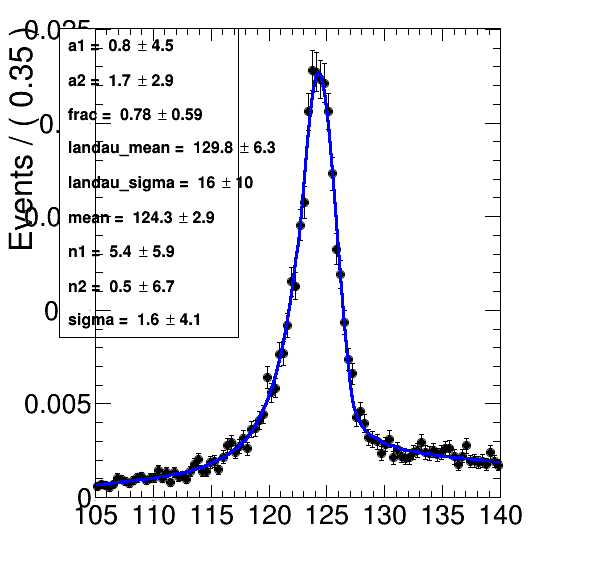
\includegraphics[width=0.32\linewidth]{Figures/Signal/fit_stage_VH_Lep_0_150_2e2mu2018.png} \\
%%\caption{The sum of the Probability density functions $f(m_{4l}|m_{H})$ for signal
%%  with {\bf $m_H$=125 \GeV} at the reconstruction level after the full lepton and event
%%  selections are applied. The distributions obtained {\bf from 13\TeV}
%%  VH MC samples are fitted with the model described in the text for
%%  $4\mu$ (left), $4e$ (center) and $2e2\mu$ (right) in the Untagged Category. The distribution show the events in the stage 1.2 bin VH\_Lep\_0\_150. %The individual
%%%  PDFs are also shown in the distinct colored plots.
%%\label{fig:sigShapeFits13TeV12xx5}}
%%\end{figure}
%%
%%\begin{figure}[!h]
%%\centering
%%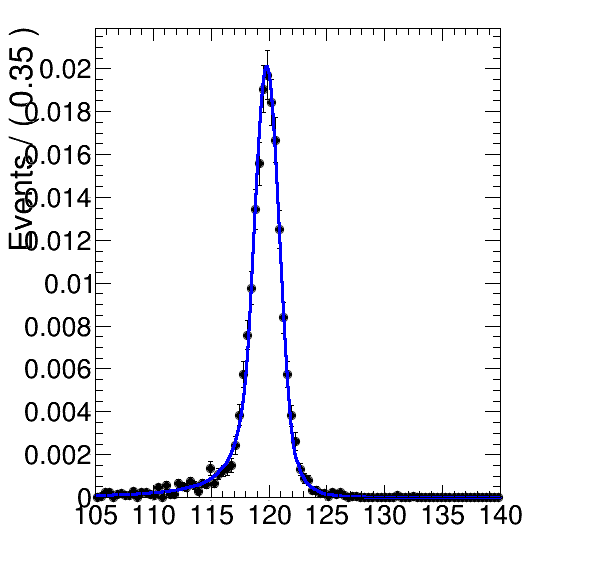
\includegraphics[width=0.32\linewidth]{Figures/Signal/simFit_VBF_2j_mjj_GT700_2j_120_4mu_2018.png} %fitM120_MOR17_ZH_2e2mu_Untagged.pdf}
%%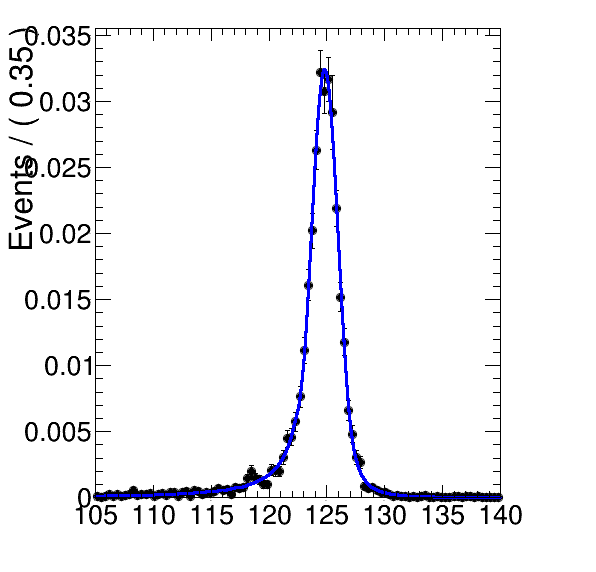
\includegraphics[width=0.32\linewidth]{Figures/Signal/simFit_VBF_2j_mjj_GT700_2j_125_4mu_2018.png} %fitM125_MOR17_ZH_2e2mu_Untagged.pdf}
%%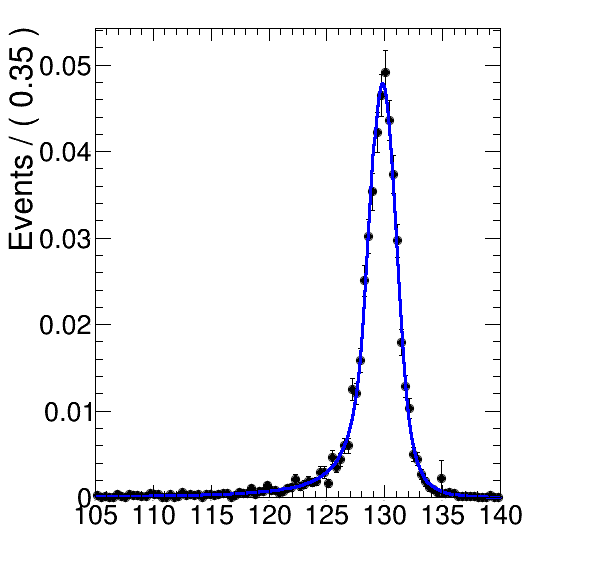
\includegraphics[width=0.32\linewidth]{Figures/Signal/simFit_VBF_2j_mjj_GT700_2j_130_4mu_2018.png} \\ %fitM130_MOR17_ZH_2e2mu_Untagged.pdf} \\
%%\caption{Simultaneous fits for  $f(m_{4l}|m_{H})$ for VBF signal with mjj above 700 GeV
%%  with {\bf $m_H$=120,125,130 \GeV} at the reconstruction level after the full lepton and event
%%  selections are applied. The distributions obtained {\bf from 13\TeV}
%%  VBF MC samples are fitted with the model described in the text for
%%  $4\mu$  events.
%%\label{fig:simFitVBF}}
%%\end{figure}
%
%%\begin{figure}[!h]
%%\centering
%%\includegraphics[width=0.32\linewidth]{Figures/SignalLineShapesPerTaggedCategory/ggH/fitM120_MOR17_ggH_4mu_Untagged.pdf}
%%\includegraphics[width=0.32\linewidth]{Figures/SignalLineShapesPerTaggedCategory/ggH/fitM125_MOR17_ggH_4mu_Untagged.pdf}
%%\includegraphics[width=0.32\linewidth]{Figures/SignalLineShapesPerTaggedCategory/ggH/fitM126_MOR17_ggH_4mu_Untagged.pdf} \\
%%\includegraphics[width=0.32\linewidth]{Figures/SignalLineShapesPerTaggedCategory/ggH/fitM120_MOR17_ggH_4mu_VBF1JetTagged.pdf}
%%\includegraphics[width=0.32\linewidth]{Figures/SignalLineShapesPerTaggedCategory/ggH/fitM125_MOR17_ggH_4mu_VBF1JetTagged.pdf}
%%\includegraphics[width=0.32\linewidth]{Figures/SignalLineShapesPerTaggedCategory/ggH/fitM126_MOR17_ggH_4mu_VBF1JetTagged.pdf} \\
%%\includegraphics[width=0.32\linewidth]{Figures/SignalLineShapesPerTaggedCategory/ggH/fitM120_MOR17_ggH_4mu_VBF2JetTagged.pdf}
%%\includegraphics[width=0.32\linewidth]{Figures/SignalLineShapesPerTaggedCategory/ggH/fitM125_MOR17_ggH_4mu_VBF2JetTagged.pdf}
%%\includegraphics[width=0.32\linewidth]{Figures/SignalLineShapesPerTaggedCategory/ggH/fitM126_MOR17_ggH_4mu_VBF2JetTagged.pdf} \\
%%\caption{Simultaneous fits for  $f(m_{4l}|m_{H})$ for ggH signal
%%  with {\bf $m_H$=120,125,126 \GeV} at the reconstruction level after the full lepton and event
%%  selections are applied. The distributions obtained {\bf from 13\TeV}
%%  MC samples are fitted with the model described in the text for
%%  $4\mu$  events. The Untagged(top), VBF1JetTagged(Middle) and VBF2JetTagged(Bottom) are shown in the respective rows.
%%\label{fig:abcsigShapeSim125}}
%%\end{figure}
